\documentclass[a4paper]{article}
%~~~~~~~~~~~~~~~~~~~~~~~~~~~~~Packages~~~~~~~~~~~~~~~~~~~~~~~~~~~~%
\usepackage[english]{babel}
\usepackage[utf8x]{inputenc}
\usepackage{booktabs}
\usepackage{tabu}
\usepackage{cancel}
%% Sets page size and margins
\usepackage[a4paper,top=2cm,bottom=2cm,left=2cm,right=2cm,marginparwidth=1.75cm]{geometry}
\usepackage{amsmath}
\usepackage{enumitem}
\usepackage{listings}
\usepackage{subfigure}
\usepackage{relsize}
\usepackage{graphicx}
%\usepackage{apacite}
\usepackage{pgfplots}
\usepackage{comment}
\usepackage{lmodern,textcomp}%For € symbol
\usepackage[colorinlistoftodos]{todonotes}
\usepackage[colorlinks=true, allcolors=blue]{hyperref}

%~~~~~~~~~~~~~~~~~~~~~~~~~~~~~Commands~~~~~~~~~~~~~~~~~~~~~~~~~~~~%

\renewcommand{\abstractname}{Summary}

%~~~~~~~~~~~~~~~~~~~~~~~~~~~~~pgfPlots~~~~~~~~~~~~~~~~~~~~~~~~~~~~%

\pgfplotsset{compat=1.8}
\usepgfplotslibrary{statistics}
%%%%%%%%%%%%%%%%%%%%%%%%%%%%%%%%%%%%%%%%%%%%%%%%%%%%%%%%%%%%%%%%%%%%

\begin{document}

\begin{titlepage}
\begin{center}
\vspace{3cm}

\Large

\vspace{2cm}

  
\includegraphics[scale=0.3]{imgs/Cherubino.jpg}

\vspace{2.5cm}

{\Huge \sc Data mining project report}

\vspace{1cm}

Maddalena Amendola

\vspace{1cm}

Daniele Gadler

\vspace{1cm}

Riccardo Manetti

\vspace{1cm}

Gemma Martini

\vfill

\today

\end{center}
\end{titlepage}

%%%%%%%%%%%%~~~~~~~~~~~~~~~~~~~~~~~~~~~~~~~~~~~~~~~~~~~%%%%%%%%%%%%

\tableofcontents
\newpage

%%%%%%%%%%%%%%~~~~~~~~~~~~~~~~~~~~~~~~~~~~~~~~~~~~~~~~~~~%%%%%%%%%%
%\author{  Group 1\\ Amendola Maddalena, Daniele Gadler, Gemma Martini, Riccardo Manetti  \\Department of Computer Science, University of Pisa \\ \date{ 1nd Semester of Academic Year 2018--2019}

%\begin{abstract}
 %  This is the abstract text
%\end{abstract}


\section{Data Understanding}

This part contains a first analysis of the data contained in the Taiwan credit card dataset. The collected data take into account users movements from April 2005 to September 2005.

\subsection{BoxPlots by Gemma}
These boxplots are created with Python and give us the chance to understand the shape of the given dataset, in order to find out possible outlayers, which may give ah hint on the many characteristics of the data.
                         %~~~~~~~~~%
\subsubsection{Age}
From this plot we can observe that age has some values below $0$. We can assume that the values allowed for this field are strictly positive.
\begin{center}
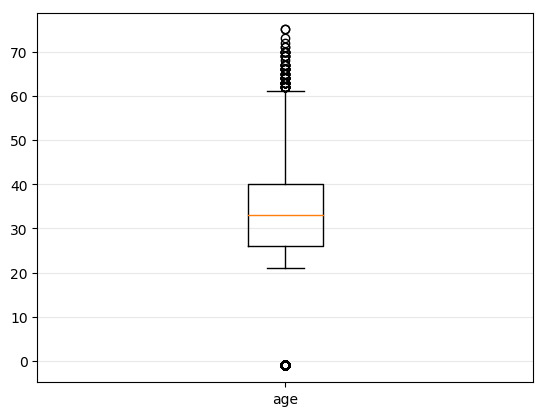
\includegraphics[width=0.9\textwidth]{../Code/boxPlotsGemma/boxplots/age.png}
\end{center}
                         %~~~~~~~~~%
\subsubsection{Limit}
Since the dataset takes into account Taiwanese dollars ($\sim 0,028$ €) plotting the boxplot in terms of multiples of the average Taiwanese income (NTD $49989$, about USD $1700$) is more informative.
\begin{center}
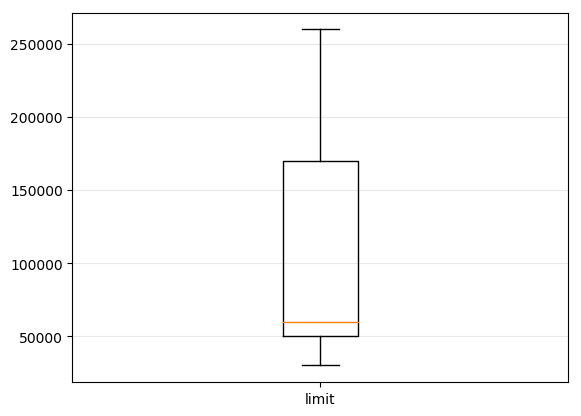
\includegraphics[width=0.48\textwidth]{../Code/boxPlotsGemma/boxplots/limit.png}
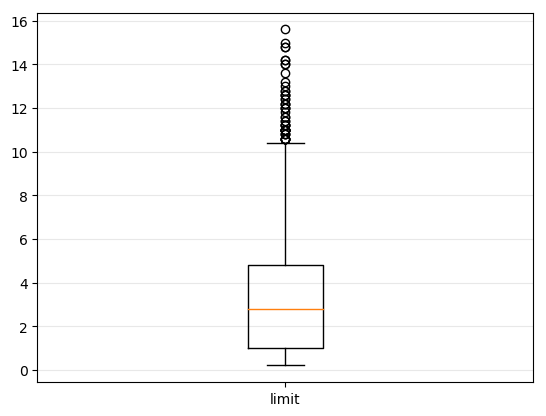
\includegraphics[width=0.45\textwidth]{../Code/boxPlotsGemma/boxplots/limitS.png}
\end{center}
From this plot we may observe that on average the limit of the credit card plafond is $2.5$ times the average income.
                         %~~~~~~~~~%
\subsubsection{Billing amount}
This values represents the balance of the bank account during the previous billing cycle.
I can't understand what all these outlayers mean!!!
\todo{I can't understand}
\begin{center}
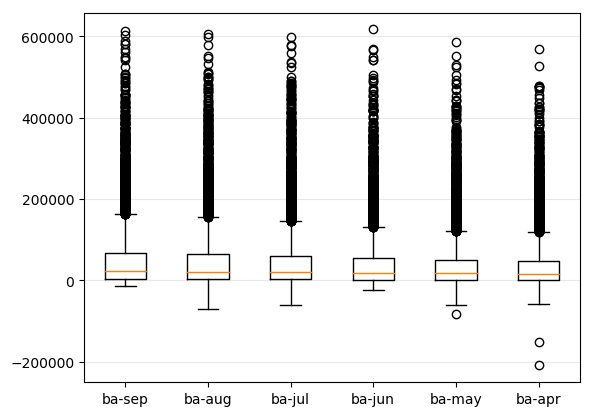
\includegraphics[width=0.9\textwidth]{../Code/boxPlotsGemma/boxplots/ba.png}
\end{center}
                         %~~~~~~~~~%
\subsubsection{Amount of previous payments}
This values tell us how much the user spent each month in the past 6 months, on a monthly basis.
\todo{Non capisco\\:-C}
\begin{center}
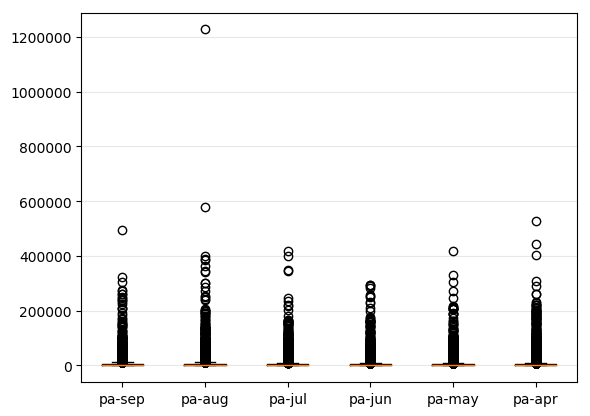
\includegraphics[width=0.9\textwidth]{../Code/boxPlotsGemma/boxplots/pa.png}
\end{center}
                         %~~~~~~~~~%
\subsubsection{Payment status}
This columns of the database contain the history of payments, more precisely:
\begin{description}
  \item[\sc Payed in time]$\rightarrow$ value $-1$

  \item[\sc Payed one month later]$\rightarrow$ value $1$

  \item[\sc Payed two months later]$\rightarrow$ value $2$

  \item[\sc Payed three months later]$\rightarrow$ value $3$

  \item[\sc Payed four months later]$\rightarrow$ value $4$

  \item[\sc Payed five months later]$\rightarrow$ value $5$

  \item[\sc Payed six months later]$\rightarrow$ value $6$

  \item[\sc Payed seven months later]$\rightarrow$ value $7$

  \item[\sc Payed eight months later]$\rightarrow$ value $8$

  \item[\sc Payed nine months later or more]$\rightarrow$ value $9$
\end{description}
\begin{center}
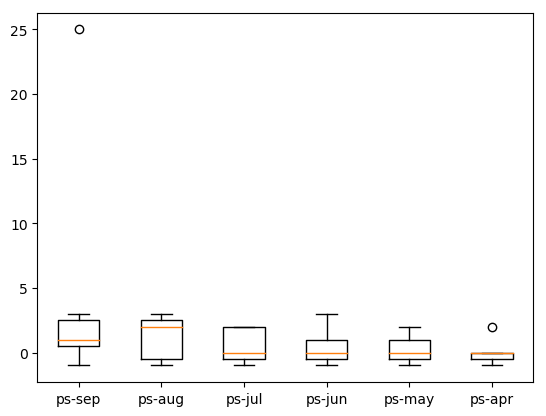
\includegraphics[width=0.9\textwidth]{../Code/boxPlotsGemma/boxplots/ps.png}
\end{center}
\todo{Direi che questo lo togliamo\\\ldots???}
\bibliographystyle{plain}
\bibliography{bibtex}

\end{document}
              
